\documentclass[border=4pt]{standalone}
\usepackage{amsmath,amssymb,tikz}
\definecolor{figB}{RGB}{31,90,166}\definecolor{figR}{RGB}{176,48,48}
\begin{document}
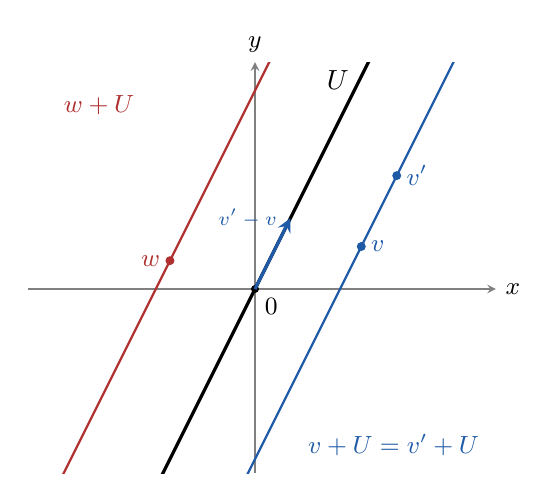
\begin{tikzpicture}[scale=0.9,>=stealth]
\draw[->,gray] (-3.2,0)--(3.4,0) node[right,black]{\small$x$};
\draw[->,gray] (0,-2.6)--(0,3.2) node[above,black]{\small$y$};
\clip (-3.2,-2.6) rectangle (3.4,3.2);
\draw[very thick,black] (-1.5,-3)--(1.7,3.4) node[pos=0.93,left]{$U$};
\draw[thick,figB] (-0.3,-3)--(2.9,3.4);
\draw[thick,figR] (-2.9,-3)--(0.3,3.4);
\fill (0,0) circle(1.6pt) node[below right]{\small$0$};
\fill[figB] (1.5,0.6) circle(1.8pt) node[right]{\small$v$};
\fill[figB] (2.0,1.6) circle(1.8pt) node[right]{\small$v'$};
\draw[->,figB,very thick] (0,0)--(0.5,1.0) node[left,xshift=-1pt]{\scriptsize$v'-v$};
\fill[figR] (-1.2,0.4) circle(1.8pt) node[left]{\small$w$};
\node[figB,anchor=east] at (3.3,-2.2){\small$v+U=v'+U$};
\node[figR] at (-2.2,2.6){\small$w+U$};
\end{tikzpicture}
\end{document}
